\section{Kaon beam analysis\label{sec-anabeam}}
In the kaon beam analysis, we identified true kaons in the kaon triggered events and obtained their momenta and trajectories. One of the most important point of the beam analysis is to assure only one beam particle is coming into the spectrometer during the time range we are interested in. Otherwise, we can not distinguish (from which beam particles a forward-going particle is generated, especially when it is neutral. %Furthermore, as already mentioned in Sec \ref{},
Furthermore, the kaon beam has microscopic beam structure which may cause fake peak structures in the $^3$He($K^-,n$) spectrum. In the current analysis, we set a time gate of forward-going particles to be the same as the TDC range of T0, $\sim$100 ns. It corresponds to down to $\sim$ 400 MeV/$c$ neutrons. To cover this time range, we selected single beam events between -30 ns and 100 ns.% with respect to a triggered particle.

An analysis procedure of the kaon beam is:
\begin{enumerate}
\item Select T0 single hit event.
\item Require that the TOF between T0 and the BHD is consistent with that of kaon beam.
\item Require that the BPC has only one track.
\item Require that BLC1 and BLC2 have only one track each.
\item Reconstruct beam momentum and check consistency with BHD hit.
\item Check consistency between BLC2 and BPC tracks.
\item Require that an extrapolation of the BPC track is on the target fiducial volume.
\end{enumerate}
The details of each step are described below.
\subsection{Kaon identification by the TOF between the BHD and T0}
Although the kaon beam is identified at the online trigger level with the AC, there are still small contaminations of pions due to the inefficiency of the AC. In addition, many events have multiple hits on the BHD and T0 as shown in Fig. \ref{fig-mulbhdt0}. We first selected T0 single-hit events to avoid beam pile-up, while we allowed multiple hits on the BHD since otherwise more than half of the statistics was lost. Instead, we developed a timing analysis method for the beam line drift chambers as described in the next section and rejected the beam pile-up event at downstream of the D4 magnet.

The associated BHD hit to the T0 hit was selected by requesting the time-of-flight between BHD and T0 to be consistent with the 1 GeV/$c$. The relative time offset and time-walk effect of the BHD was calibrated with respect to T0 segment \#3 by using pions with a fixed flight length of 7.7 m and a fixed beam momentum of 1 GeV/$c$. A typical TOF resolution of 160 ps ($\sigma$) was obtained for 1 GeV/$c$ pions, where the flight length deviation from the central trajectory is not taken into account. A typical TOF spectrum is shown in Fig. \ref{fig-tofk}. The kaon selection gate was defined by the 3$\sigma$ of the kaon peak, where the TOF resolution for 1 GeV/$c$ was evaluated to be 195 ps($\sigma$). The additional deterioration of the resolution is due to the ignorance of the $\sim$ 2\% beam momentum bite.
\begin{figure}[]
\begin{center}
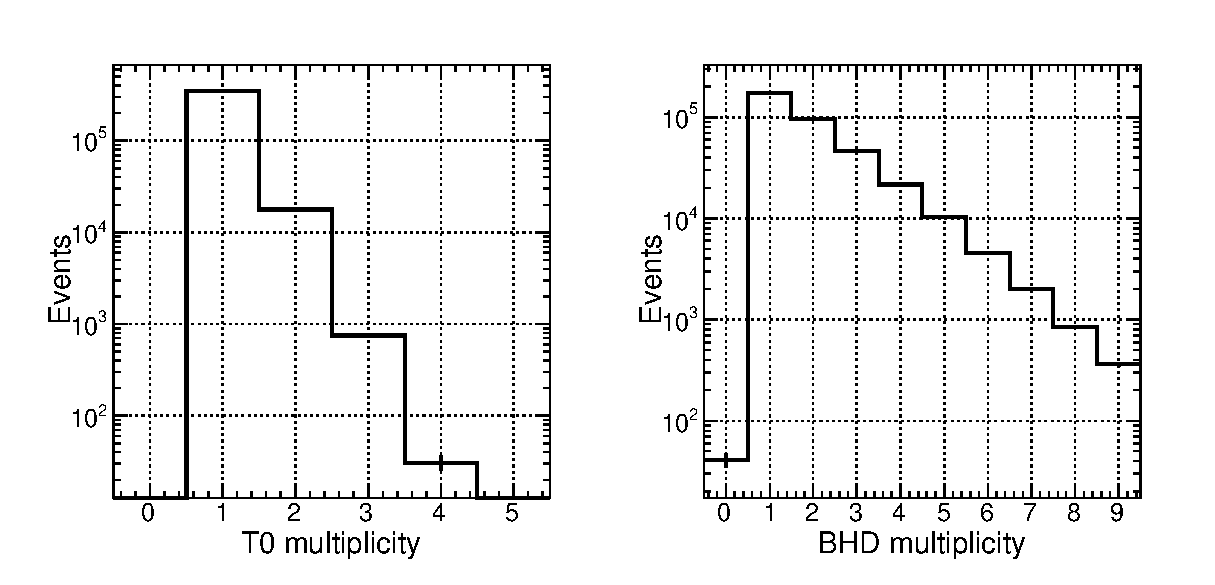
\includegraphics[width=\columnwidth]{./fig/mul-bhdt0.eps}
\caption[Multiplicity of T0 and the BHD.]{Multiplicity of (left) T0 and (right) the BHD for the unbiased-kaon beam. The T0 single-hit is required in the right figure.}
\label{fig-mulbhdt0}
\end{center}
\end{figure}  
\begin{figure}[]
\begin{center}
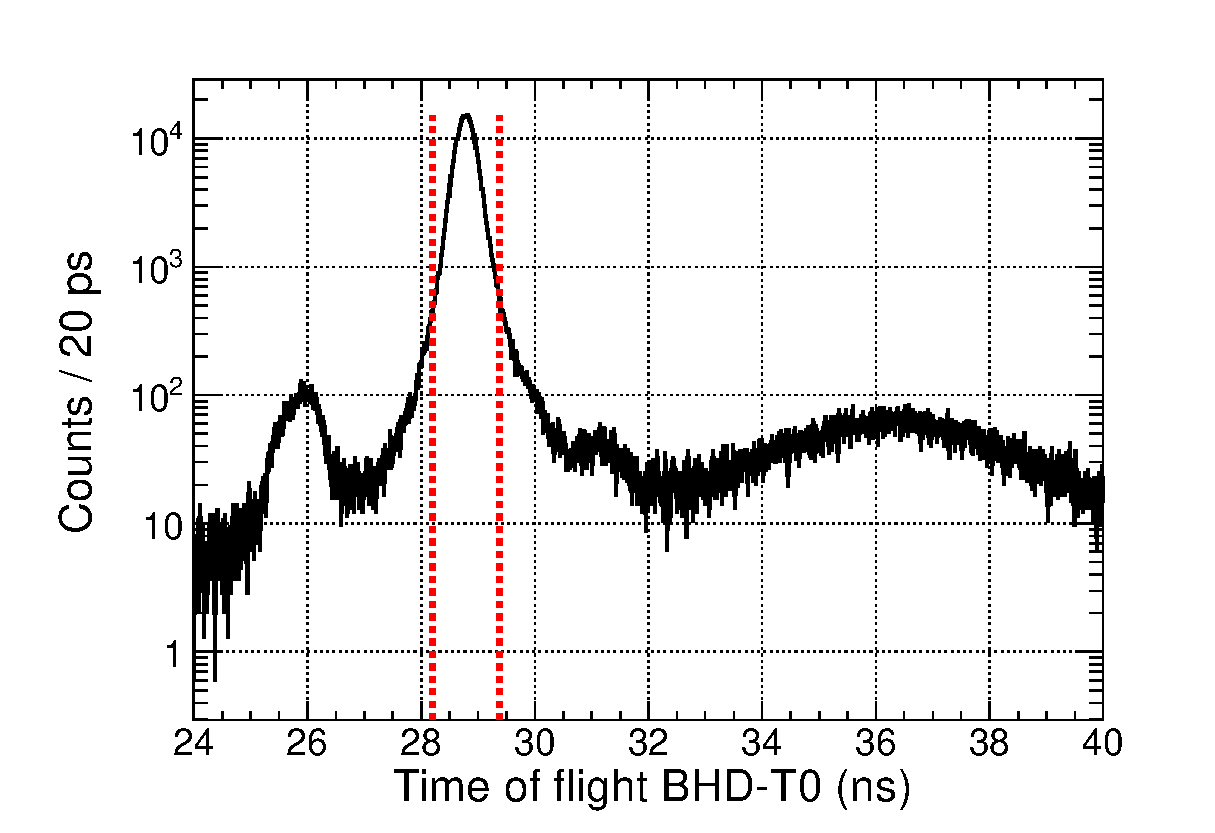
\includegraphics[width=10cm]{./fig/tofk.eps}
\caption[Time-of-flight distribution between the BHD and T0.]{Time-of-flight distribution between the BHD and T0. Unbiased kaon trigger data is used. Multiple hits on the BHD are allowed. A peak around 29 ns corresponds to the kaon timing and the red dot lines show the kaon selection region. A peak around 26 ns is contributed from pion contamination. A bump above 33 ns is considered due to the beam pile-up events.}
\label{fig-tofk}
\end{center}
\end{figure}  
\subsection{Beam-line drift chamber analysis}

\subsubsection{Conversion to the hit position}
The TDC data of drift chambers is converted to drift time information. Assuming that the beam particles pass through the chambers at right angles and are uniformly distributed in each cell, a conversion relation between a drift time and a drift length can be obtained from the integral of the time distribution as shown in Fig. \ref{fig-bldcdtdx}(top and middle). The conversion relations were obtained wire by wire with the kaon beam, and a relative offset of each wire was adjusted by using a peak position in the differentiated time spectrum as shown in Fig.~\ref{fig-bldcdtdx}(bottom).

\begin{figure}[]
\begin{center}
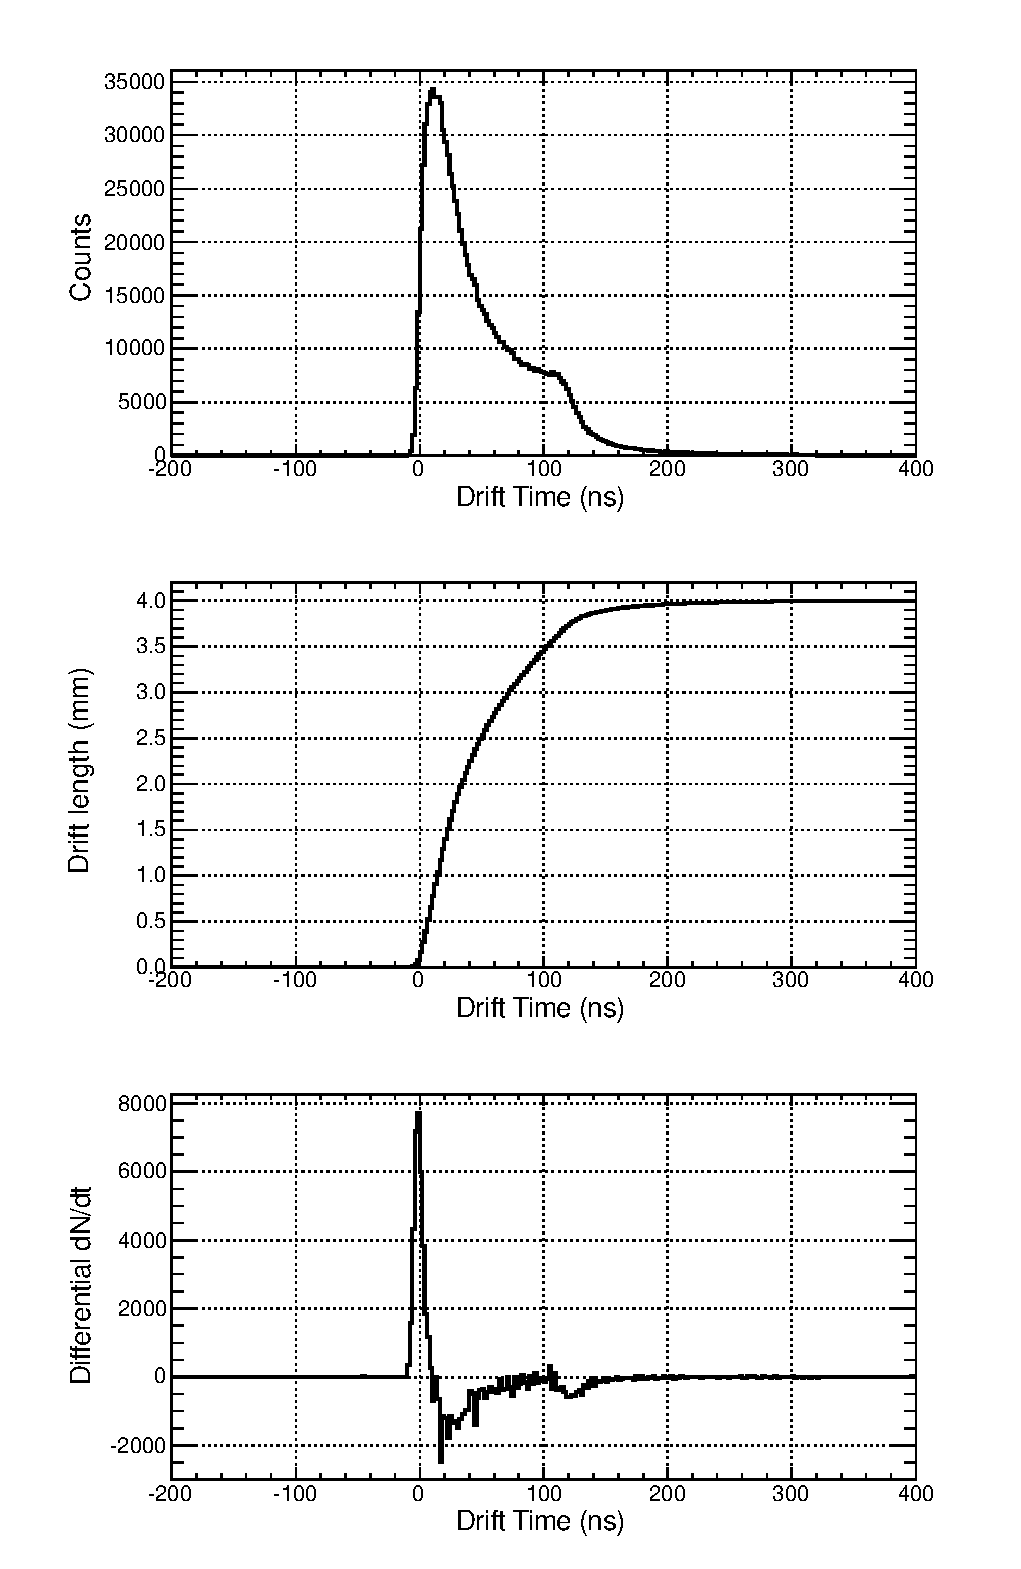
\includegraphics[width=12cm]{./fig/bldcdtdx.eps}
\caption[Timing distribution, integrated timing spectrum, and differential timing spectrum of a typical wire in BLC1.]{(top) Timing distribution of a typical wire in BLC1. (middle) Integrated timing spectrum. The maximum was normalized by the maximum drift length. (bottom) Differential of the timing distribution. The peak position was used to adjust the relative timing offset.}
\label{fig-bldcdtdx}
\end{center}
\end{figure}  

\subsubsection{Linear tracking}
A hit position in each plane can be calculated from a wire position and a drift length, but there is still ambiguity in the drift direction. For a given set of the hits, all combinations of the drift directions were examined and the combination which gives minimum $\chi^2/ndf$ was selected. The $\chi^2/ndf$ in the 3 dimensional linear fitting is defined as,
\begin{eqnarray}
\chi^2/ndf&=& \frac{1}{N-4}\sum_i^N\left(\frac{x'_i-f(z_i)}{\sigma_i}\right)^2,\\
f(z)&=& \cos\theta(a+zb)+\sin\theta(c+zd), \label{eq-trackrot}
\end{eqnarray}
where $N$ is the number of the given hits, $x'$ is the positions perpendicular to the wire and the beam direction,  $f(z)$ is the calculated position in a rotated plane with an angle of $\theta$, and $\sigma$ is the assumed position resolution. We employed the position resolutions in Table \ref{tab-chmperformance} for the calculation. The four parameters a, b, c, d in eq. \ref{eq-trackrot} at the minimum $\chi^2$ are analytically calculated for the given set of the hits.

\subsubsection{Timing analysis}
Since the gate windows for the TDCs were set to $\sim$500 ns, there were many multi-track events which had multi hits in the beam line drift chambers. To select a correct set of the hits and to reject tracks out of the triggers particle, a timing analysis was introduced. Although a single-hit-timing information is useless due to large drift-time distribution of $\sim$100 ns, the timing of the particle passage can be deduced by using hits of paired plane, such as $XX'$.

All beam-line chambers  consist of pairs of staggered planes by a half of the cell size. Therefore, for the correct set of the hits,  a sum of the drift lengths of the paired hits should be approximately the cell width, i.e., the drift times in the paired planes should be correlated. Figure \ref{fig-dctime}(top) shows the relation between a differential and an average of drift times in the paired planes. Here, single-track events were selected to ensure the hits were generated by the trigger particle. The correlation in Fig. \ref{fig-dctime}(top) is due to the asymmetric conversion relation between the drift time and the drift length (Fig, \ref{fig-bldcdtdx}(middle)). After correcting the correlation as shown in Fig. \ref{fig-dctime}(b), the corrected average drift-time gives the timing of the particle passage. The correction relations were determined plane by plane. Note that when the paired-hits search was failed, then those paired planers were excluded from the timing analysis.

\begin{figure}[]
\begin{center}
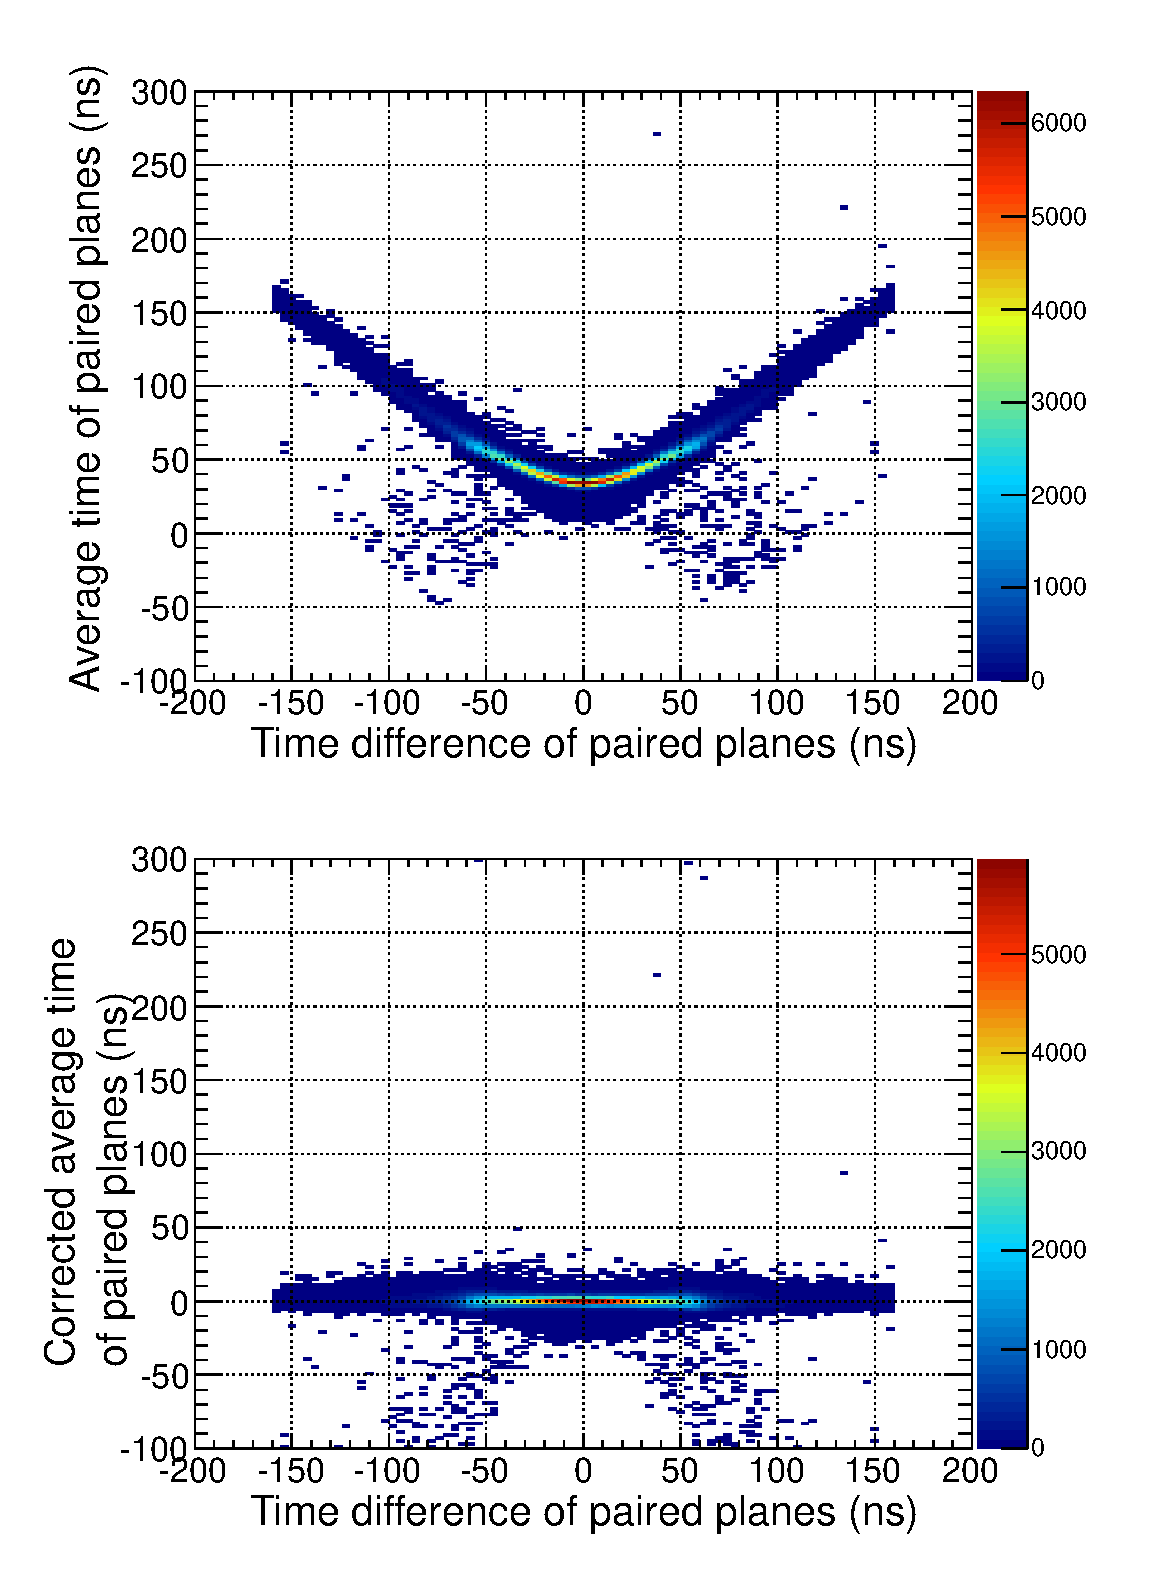
\includegraphics[width=12cm]{./fig/dctime.eps}
\caption[Typical correlation of the time difference and the average time of paired plane.]{(top) Typical correlation of the time difference and the average time of two neighboring wire hits. Single track event at 0 ns is selected with other chambers and counters. (bottom) After the correction. }
\label{fig-dctime}
\end{center}
\end{figure}  

\subsubsection{Track search at a local level}
At first, tracks were searched at a local level, BLC1, BLC2 and the BPC, independently. All possible candidates of hit combinations were examined. For BLC1 and BLC2, a candidate was required to have hits in more than 5 planes out of 8 planes in each of U and V planes. All 8 planes were requested to have hits for the BPC because of the lack of redundancy. The number of candidates was reduced with the help of timing analysis and pre-fitting with a MWPC mode, namely without drift time consideration. Then a hit combination with a minimum $\chi^2/ndf$ was selected as a first track. The procedure was iteratively done with hits not included in reconstructed tracks, until we have no more hits enough to reconstruct an additional track. 

\subsubsection{Definition of a good track}
The reconstructed tracks were further examined. First, the $\chi^2/ndf$, whose typical distributions are shown in Fig. \ref{fig-bldcchi}, was requested to be less than 10. To avoid beam pile-up events, single track event within the timing window of (-30,100) ns was selected as shown in Fig.\ref{fig-bldctime}. In addition, the tracks were also required to be associated to the trigger timing. The timing windows of the trigger association were defined to be (-5,5) ns and (-10,10) ns for the BLCs and the BPC, respectively. Typical track multiplicities are shown in the right of Fig. \ref{fig-bldctime} for different timing windows.

\begin{figure}[]
\begin{center}
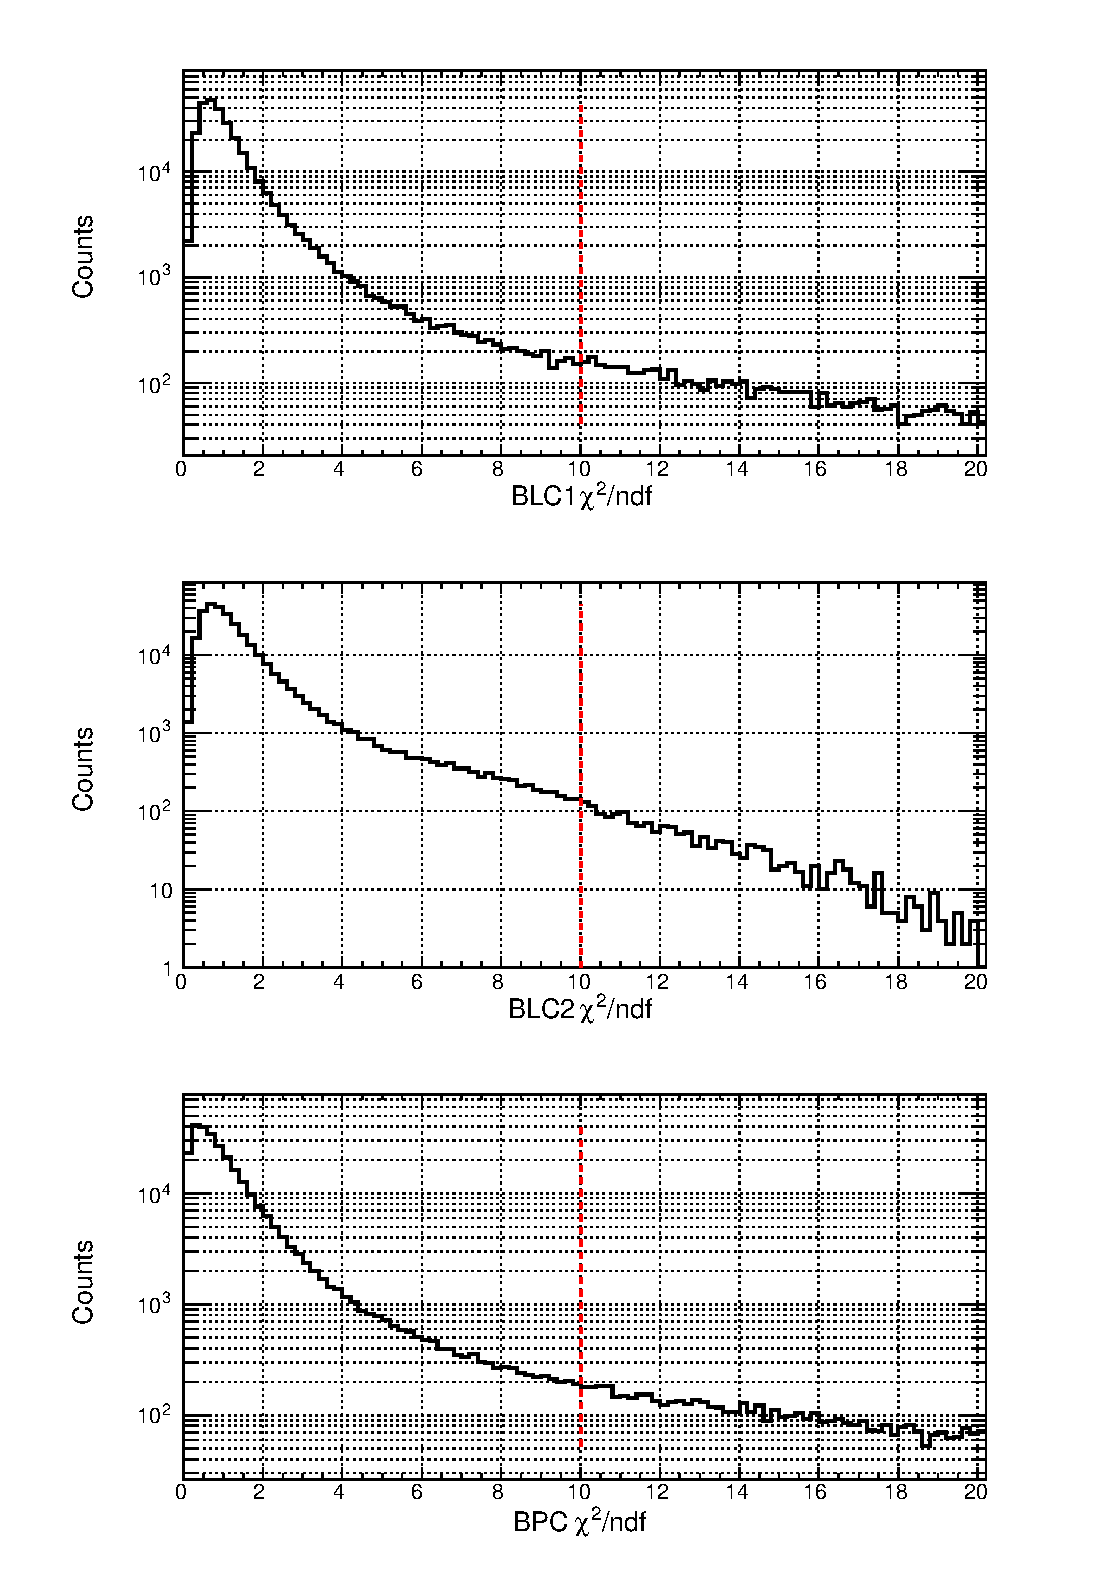
\includegraphics[width=12cm]{./fig/bldc-chi2.eps}
\caption[$\chi^2/ndf$ distributions of BLC1, BLC2 and the BPC. ]{$\chi^2/ndf$ distributions of BLC1, BLC2 and the BPC. $\chi^2/ndf<$10 tracks were accepted. }
\label{fig-bldcchi}
\end{center}
\end{figure}  

\begin{figure}[]
\begin{center}
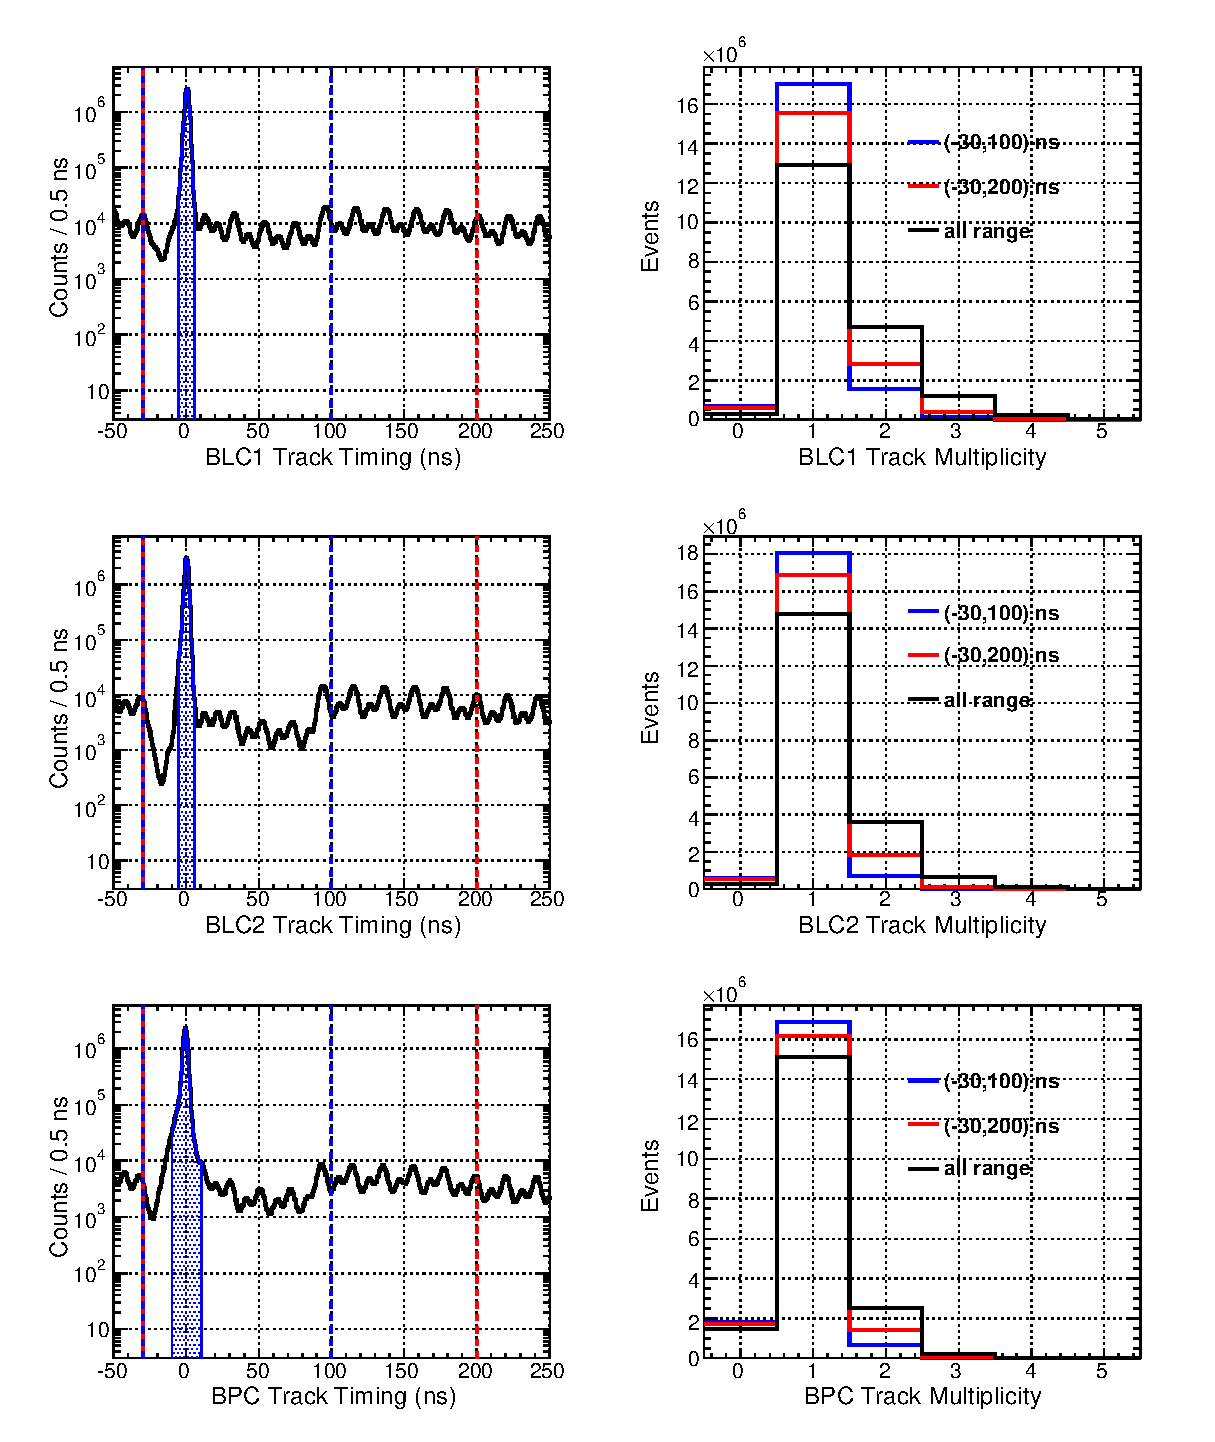
\includegraphics[width=14cm]{./fig/chmtime.eps}
\caption[Track timing distributions and track multiplicities of the beam-line drift chambers.]{(left) Track timing distributions. T0 single hit and at least 1 CDC track were already required. Due to the T0 single hit selection, pile-up events in the T0 TDC range of (-20, 80) ns was reduced. The largest peak around 0 ns corresponds to the triggered particle and others are pileup events. The red dotted lines give the region for the multiplicity counting and the trigger associated windows were defined as blue hatches. (right) Track multiplicities with different timing windows. The (-30,100) ns timing window is employed in the current analysis.}
\label{fig-bldctime}
\end{center}
\end{figure}  

%\end{enumerate}
\subsection{Performance of the beam line drift chambers}
\subsubsection{Position resolution}
An intrinsic position resolution of the plane is related to the residual distribution. The residual distribution for all wires in the plane was fitted with a Gaussian and the resultant Gaussian sigma is converted to the intrinsic position resolution by using a factor calculated with the geometry of the chamber.  Typical resolutions appear in Table \ref{tab-chmperformance} are averages of the resolutions of all planes in the drift chambers.  
%The time dependency of the same quantity is plotted in Fig. \ref{} for BLC1, BLC2 and BPC.
\subsubsection{Timing resolution}
Since the typical drift velocity under the present operational condition is $\sim$ 50 $\mu$m/ns, the timing resolutions in the paired plane analysis are expected to be a few ns. The time resolution of a paired planes were obtained to be $\sim$ 3 ns from the Y-projected distribution of Fig. \ref{fig-dctime}(bottom). The time resolutions of a track were evaluated using the 0 ns peaks in Fig. \ref{fig-bldctime}(left). The obtained resolutions are summarized in Table \ref{tab-chmperformance}.

\subsubsection{Tracking efficiency}
A tracking efficiency of the beam line drift chamber was evaluated by requiring single track in each of other two beam-line drift chambers. For the BPC, a track extrapolated from BLC2 was requested to be at the center of the BPC. Note that plane efficiencies were $>$99\% for all planes in all beam line chambers, except for plane \#5 of the BLC2b and plane \#4 of FDC1, which have a dead wire, respectively. 

Typical values of the resultant efficiencies are listed in Table \ref{tab-chmperformance}.% and the run dependence of tracking efficiencies are show in Fig \ref{}.

\begin{table}[]
\caption{Typical performance of the drift chambers evaluated with unbiased kaon beam data.}
\begin{center}
\begin{tabular}{l|cccccc} 
\hline\hline													
	&	BLC1a	&	BLC1b	&	BLC2a	&	BLC2b	&	BPC	&	FDC1	\\
\hline													
\shortstack{Position resolution\\~~~of a plane (mm)}	&	130	&	180	&	170	&	180	&	110	&	120	\\
\shortstack{Timing resolution\\~~~of paired planes (ns)}	&	2.8	&	3.3	&	2.5	&	2.8	&	2.7	&	—	\\
\shortstack{Timing resolution\\~~~of a track (ns)}	&	\multicolumn{2}{c}{1.4}			&	\multicolumn{2}{c}{1.2}			&	1.4	&	—	\\
Tracking efficiency (\%)	&	\multicolumn{2}{c}{98.4}			&	\multicolumn{2}{c}{97.2}			&	98.3	&	97.4	\\
\hline\hline												
\end{tabular}
\end{center}
\label{tab-chmperformance}
\end{table}%

\subsection{Beam momentum reconstruction}
The BLC1 and BLC2 tracks were connected using a second-order transfer matrix calculated by TRANSPORT code\cite{Anonymous:M8WJFLy5} with an additional parameters for the beam momentum. The definition of the $\chi^2$ was essentially the same as Eq. \ref{eq-trackrot}, except that we have an additional degree of freedom of the beam momentum. The minimization of the $\chi^2$ was performed with the help of a minimization code, TMinuit\cite{James:1975he}.

The resultant $\chi^2$ distribution is shown in Fig. \ref{fig-d5chi2}. The events with $\chi^2$ $<$ 20 were accepted.% and their momentum distribution is shown in Fig. \ref{fig-d5mom}. 

\begin{figure}[]
\begin{center}
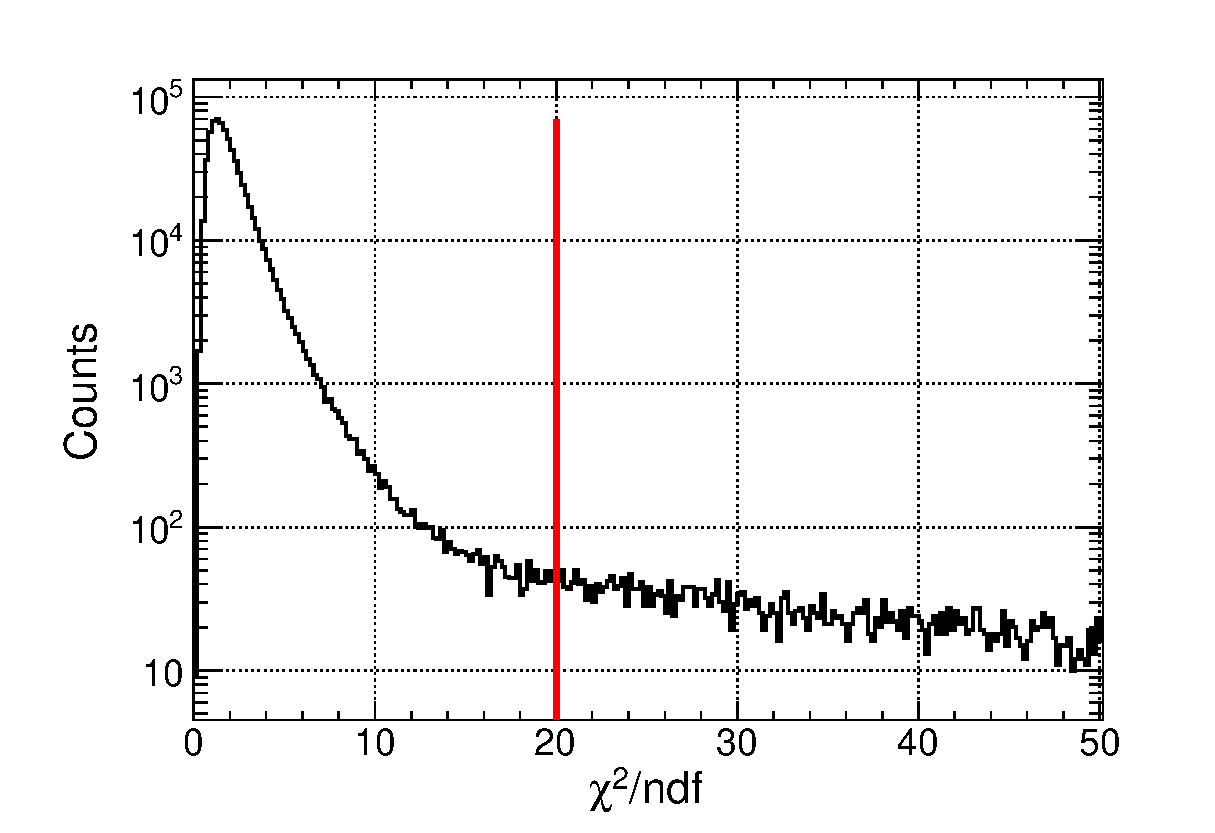
\includegraphics[width=12cm]{./fig/d5chi2.eps}
\caption[$\chi^2/ndf$ distribution in the fitting to connect BLC1 and BLC2 track. ]{$\chi^2/ndf$ distribution in the fitting to connect BLC1 and BLC2 track. $\chi^2/ndf<$20 was accepted.}
\label{fig-d5chi2}
\end{center}
\end{figure}  


\subsubsection{Comparison with the forward spectrometer\label{sec-beammom}}
To evaluate the absolute beam momentum, we used proton beam data to the PC. The proton beam momentum just upstream of T0 was analyzed with a TOF method between T0 and the PC, and was used as the reference. The details of an analysis method of a forward charged particle is described in Appendix B. Note that the momentum scale of the forward charged spectrometer was essentially determined by the detector geometry.

Figure \ref{fig-beamthrough} shows the comparison of the reconstructed momentum of the proton beam by the two spectrometers, beam line spectrometers (D5) and the forward charged particle spectrometer (PC), where a systematic difference between the two methods was observed. If it was due to the mis-alignment of the forward spectrometer, we need to modify the position of the PC by 10 cm order. It is more natural to suspect the beam spectrometer, which had many uncertainty in the magnetic field of the D5 and the relative positions of the drift chambers. Therefore, a linear correction function shown in Fig. \ref{fig-beamthrough}(left) was applied for the momentum reconstructed with the beam line spectrometer. Figure \ref{fig-beamthrough}(right) shows the distribution of the difference of the reconstructed momenta with the two methods after the correction. The distribution can be interpreted as a squared sum of the momentum resolution of the two methods. 

The momentum resolution of the T0-PC system was evaluated with a simulation to be 3.4 $\pm$ 0.3 MeV/$c$ for a proton beam with a momentum of 1 GeV/$c$. The simulation included the effects of multiple scatterings, energy losses and other physics processes. Realistic resolutions for drift chambers in Table \ref{tab-chmperformance} were also considered. The error was evaluated from the uncertainty in the intrinsic timing resolution of T0 and the PC. They were measured only with cosmic rays, namely minimum ionizing particles (MIPs), while a 1 GeV/$c$ proton deposits 1.5 times more energy and thus resulting in a better timing resolution. Here we assumed 0 and 25\% improvement of the timing resolution at maximum for 1 GeV/$c$ protons compared to MIPs. The average and the deviation of the resulting two momentum resolutions were employed as the resolution of the system and its error, respectively.

From the distribution in Fig. \ref{fig-beamthrough}(right) and the evaluated momentum resolution of the T0-PC system, the momentum resolution of the beam spectrometer was obtained to be 2.0 $\pm$ 0.5 MeV/$c$. The precision of the absolute momentum scale should be at the same level of that of the T0-PC system, which was evaluated to be $\sim$2 MeV/$c$ in Appendix B. The absolute scale will be further discussed as the missing mass scale in Sec. \ref{sec-scale}.

Figure \ref{fig-d5mom2} shows the kaon beam momentum distribution. % after the correction described above.
\begin{figure}[]
\begin{center}
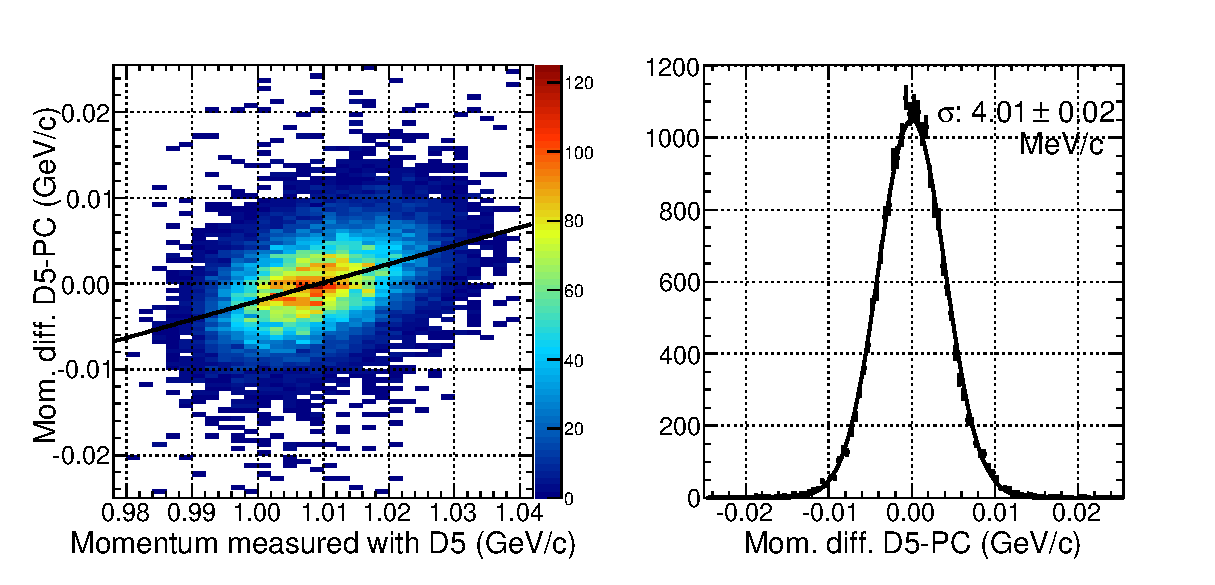
\includegraphics[width=\columnwidth]{./fig/pc-beamthrough.eps}
\caption[Comparison of the two reconstructed momenta with the beam-line spectrometer and the forward TOF spectrometer. ]{(left) Momentum dependence of the difference of reconstructed momenta with two different spectrometer, the beam-line spectrometer(D5) and the forward charged spectrometer(PC). (right) Distribution of the momentum difference after the correction with a linear function drawn in (left) with a black solid line.}
\label{fig-beamthrough}
\end{center}
\end{figure}  

\begin{figure}[]
\begin{center}
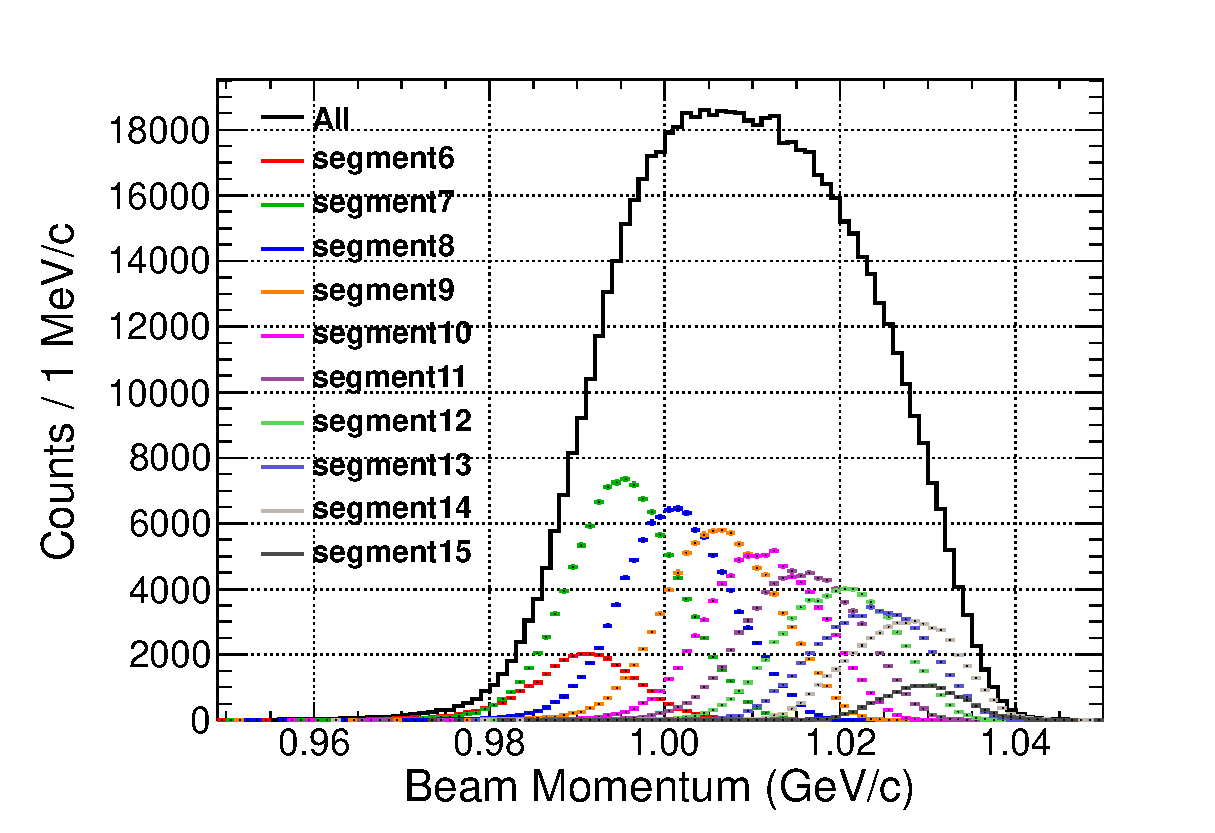
\includegraphics[width=12cm]{./fig/d5mom2.eps}
\caption[Distribution of the reconstructed beam momentum. ]{Distribution of the reconstructed beam momentum. Colored histograms represents the momentum distribution at each BHD segment.}
\label{fig-d5mom2}
\end{center}
\end{figure}  

\subsection{Event selection}
\subsubsection{Correlation between momentum and BHD hit}
Since the BHD position is located on a dispersive point, there is a clear correlation between the reconstructed kaon momentum and a hit segment of the BHD, which can be interpreted as the $x$ position at the BHD as shown in Fig. \ref{fig-bhdmom}. Fake combinations between a BHD hit and a BLC1-BLC2 track, mainly caused by kaon decays and pile-up particles, were rejected by applying three sigma cut on the distributions.

\begin{figure}[]
\begin{center}
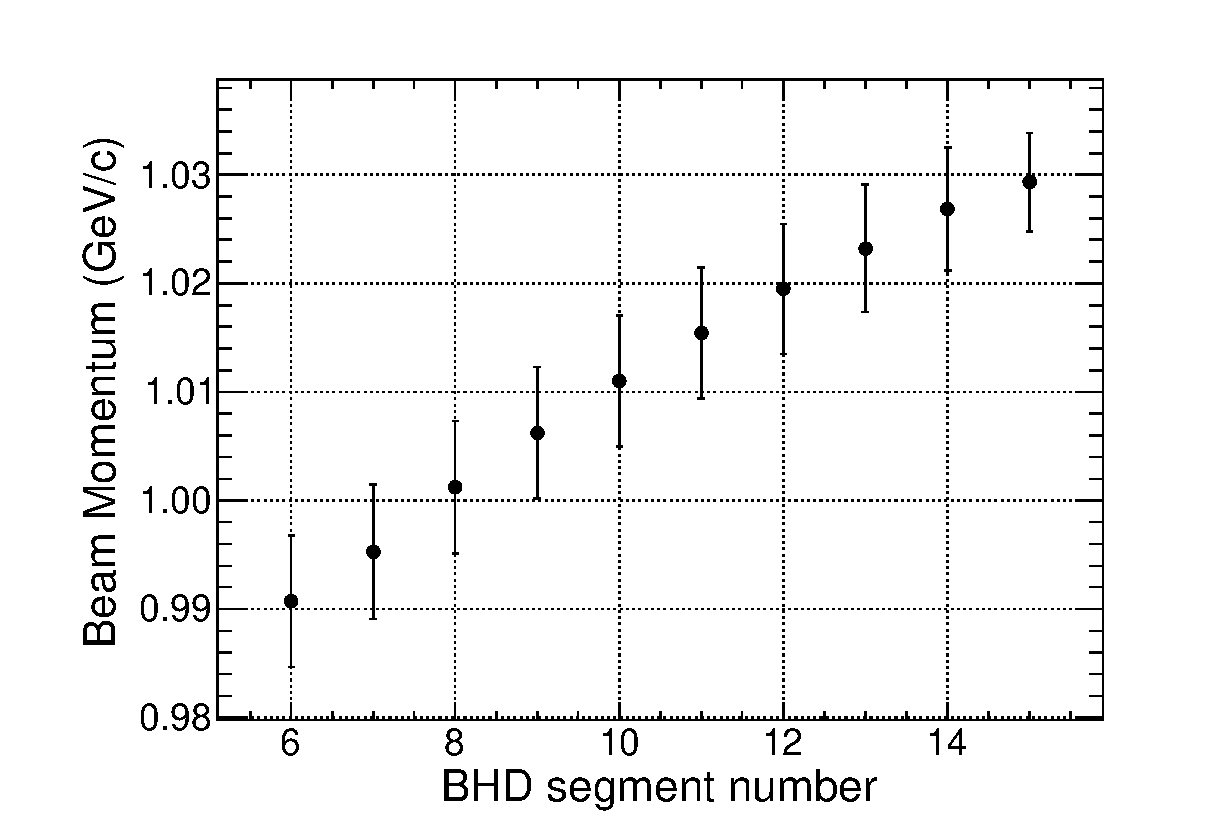
\includegraphics[width=12cm]{./fig/bhdmom.eps}
\caption[The relation between the hit segment of the BHD and the momentum distribution.]{The relation between the hit segment of the BHD and the momentum distribution. The mean value and the error bar represent the mean and sigma obtained by the Gaussian fitting of each colored distribution in Fig. \ref{fig-d5mom2}, respectively.}
\label{fig-bhdmom}
\end{center}
\end{figure}  

\subsubsection{Track matching between BLC2 and the BPC}
A portion of kaons also decay or react after identified by the AC. To reduce such events and to ensure the BPC track is the kaon beam, the track matching between BLC2 and the BPC was examined. Figure \ref{fig-blc2bpc} shows position and direction matchings, where three sigma cuts were applied for the BLC2-BPC track selection.

\begin{figure}[]
\begin{center}
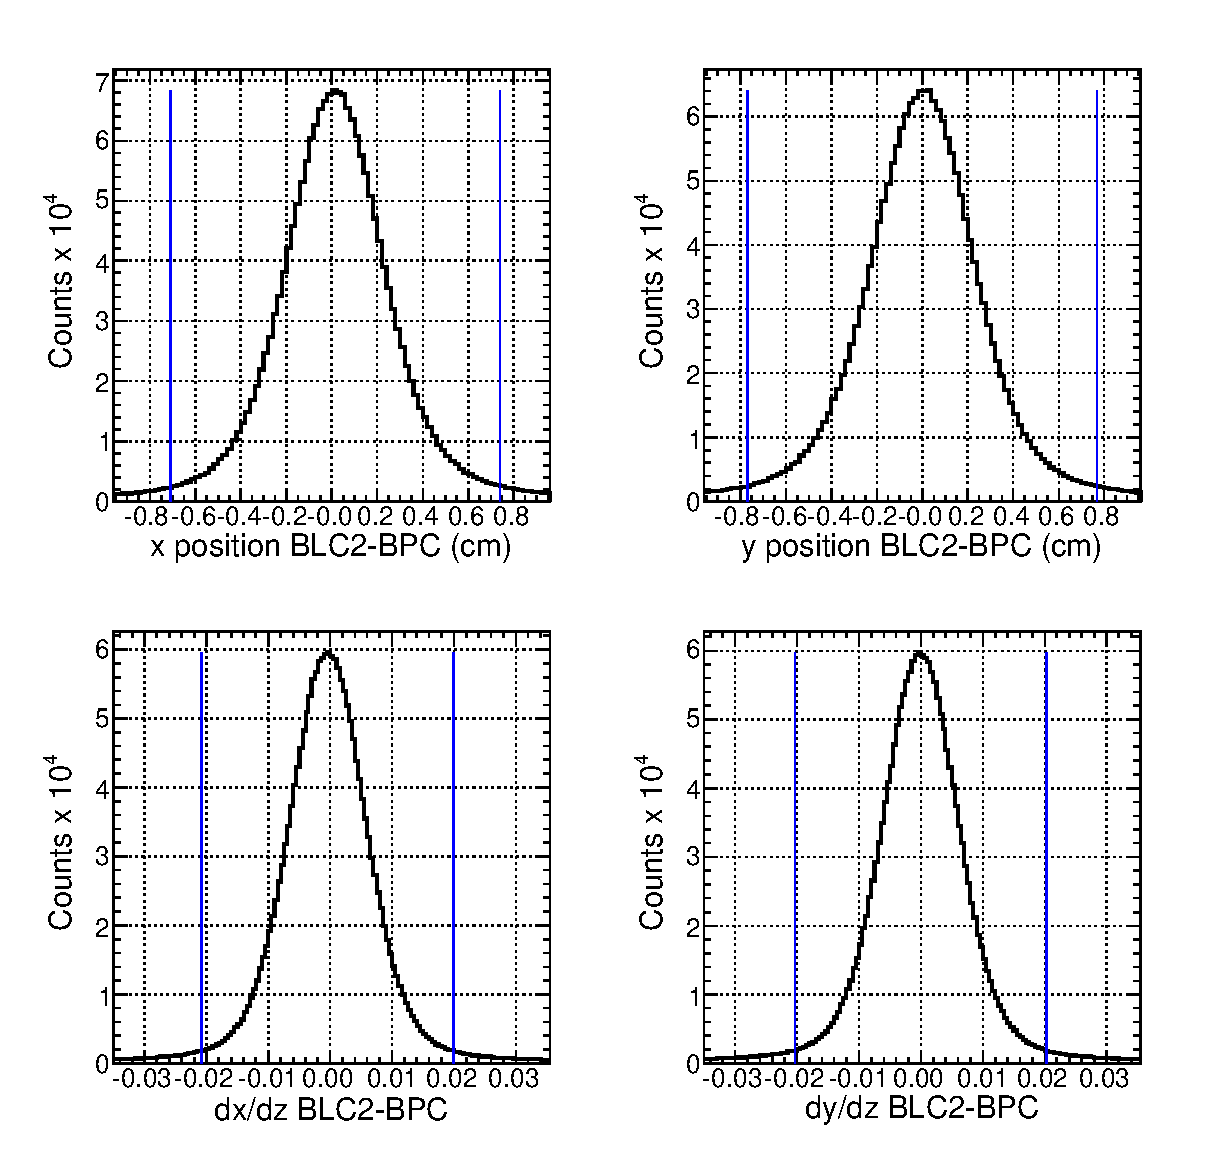
\includegraphics[width=14cm]{./fig/blc2bpc.eps}
\caption[Track matching between BLC2 and the BPC.]{Track matching between BLC2 and the BPC at $z=-75$ cm. The two blue vertical lines in each histogram define the accepted region.}
\label{fig-blc2bpc}
\end{center}
\end{figure}  

\subsubsection{Beam profile at the final focus point}
Figure \ref{fig-ffprof}(a) shows the kaon beam distribution at the final focus point evaluated by extrapolations of the BPC tracks. The target cell shape was clearly seen in Fig. \ref{fig-ffprof}(b), where the CDH trigger was requested. Although the beam spot size was a bit larger than the target size and the target cell was displaced from the center of the CDS, the position of the beam was well controlled on the target center. Note that the fiducial volume was defined in three-dimensionally as described in Sec.~\ref{sec-fiducial}.

\begin{figure}[]
\begin{center}
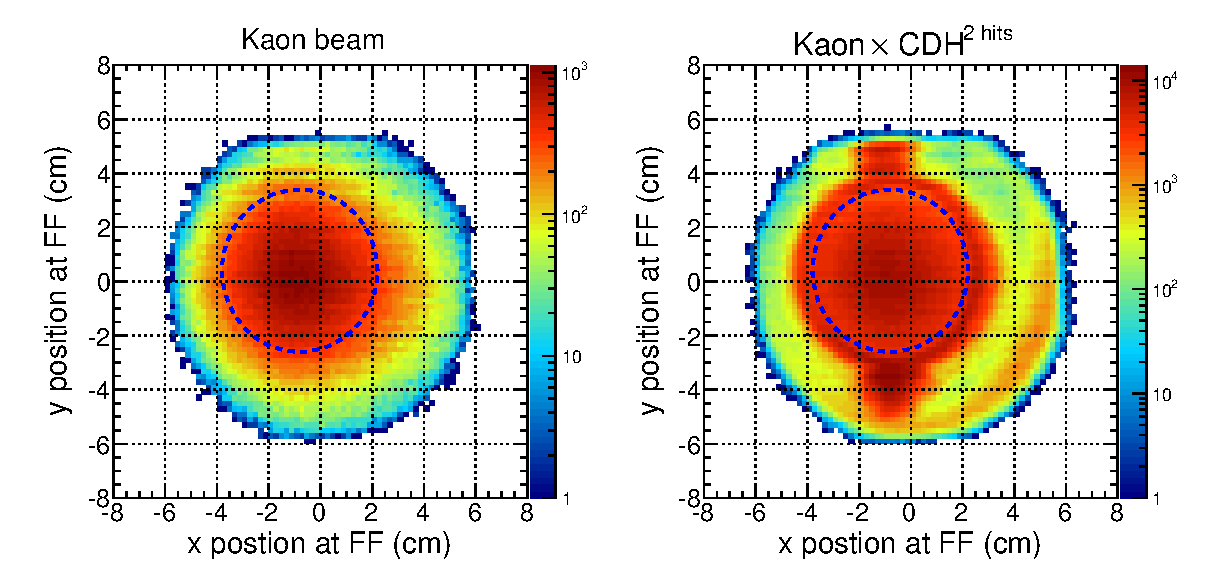
\includegraphics[width=\columnwidth]{./fig/ffprof.eps}
\caption[Kaon beam profile at the FF.]{Kaon beam profile at the FF (left) without any bias and (right) CDH 2 hits was required at a trigger level. The dotted circles represent the $xy$ fiducial region at the FF.}
\label{fig-ffprof}
\end{center}
\end{figure}  

\subsection{Luminosity evaluation\label{sec-luminosity}}
\subsubsection{Decay and reaction loss}
With the event selections described above, the kaon was guaranteed to be alive at the final plane of the BPC. Although the DEF hit was required at the trigger level, charged particles from kaon decays or reactions often hit on the DEF.

Therefore, we evaluated the decay and reaction loss probabilities between the plane 8 in the BPC ($z=-$18 cm) and the FF ($z$=0). For a fixed beam momentum of 1 GeV/$c$, kaon decay loss was calculated to be 2.4$\%$ with $c\tau$=3.712 m. The relative position uncertainty of $\sim$ 1 cm between the BPC and the FF gives 0.2\% systematic error. The effect of the $\sim$2\% beam momentum bite is smaller than 0.1\%. 
For the estimation of the reaction loss, the elementally $K^-N$ reaction cross section was simply scaled by the size of nucleus $A^{2/3}$. The materials considered in the evaluation were the DEF, the cap of the target vessel, the radiation shield and the target cell window. The total thickness was $\sim$0.67 g/cm$^2$ as summarized in Table \ref{tab-matbeam}. The reaction loss rate was obtained to be 0.7\% and the uncertainty of the estimation for the $K^-N$ reaction cross section was considered to give 20\% systematical error.

\subsubsection{Number of the target particle}
We defined the fiducial volume length as 10 cm, which is actually defined in three-dimensionally as shown in Fig. \ref{fig-cdcvertex}. The path length of the kaons in the fiducial volume was evaluated from the extrapolation of the BPC tracks using the unbiased kaon beam data. The normalized path length was obtained to be 10.03$\pm$0.02 cm. The error is evaluated by the time fluctuation during the production run.

The density of the helium-3 target was evaluated to be 0.0810$\pm$0.0002 as described in Sec. \ref{sec-target}.

\subsubsection{Kaon flux and integrated luminosity}
Finally, total kaon beam flux and the integrated luminosity used in the analysis was evaluated based on a scaler count of the kaon beam trigger, the analysis efficiency in the event selection, and the various factors discussed above. The event selection criteria and corresponding efficiencies are summarized in Table \ref{tab-beamflux}. 
The total kaon beam number incident on the target was evaluated to be ($3.31\pm0.06) \times 10^9$ and the integrated luminosity was to be 540$\pm$10 $\mu$b$^{-1}$. The errors associated to the kaon beam selection should be basically cancelled in calculating cross sections since the same event selections were applied in the data analysis and the integrated luminosity evaluation. However, time fluctuations of those survival rates, given as relative uncertainties in Table \ref{tab-beamflux}, were considered not to be cancelled.%, which was xx\% of the number of hardware kaon triggers.

\begin{table}[]
\caption[Typical values of the survival rate at each step of beam selection. ]{Typical values of the survival rate at each step of beam selection. Relative uncertainties of the survival rates in the kaon beam selection were determined by the fluctuations during the experimental period.}
\begin{center}
\begin{tabular}{l|ccc} 
\hline\hline					
		&	number		&	survival rate	&	relative uncertainty (\%)	\\
\hline									
Scaler number		&	7.52	$\times 10^9$	&	1	&		\\
\hline									
T0 single hit		&			&	0.950	&	0.3	\\
TOF kaon		&			&	0.973	&	0.2	\\
BPC single track		&			&	0.916	&	0.4	\\
BLC1\&2 single track		&			&	0.868	&	1.2	\\
BLC2-BPC connection		&			&	0.890	&	0.4	\\
momentum reconstruction		&			&	0.991	&	0.1	\\
									
\hline									
Fiducial selection at FF		&			&	0.696	&	1.0	\\
decay loss		&			&	0.976	&	0.2	\\
reaction loss		&			&	0.993	&	0.3	\\
\hline									
Total		&	3.31	$\times 10^9$	&	0.441	&	1.7	\\
\hline\hline									
Density	(g/cm$^3$)	&	0.081		&		&	0.3	\\
Thickness	(cm)	&	10.03		&		&	0.2	\\
\hline\hline												
Luminosity	($\mu$b$^{-1}$)	&	540		&		&	1.9	\\
\hline\hline												
\end{tabular}
\end{center}
\label{tab-beamflux}
\end{table}%
